\documentclass[10pt,a4paper]{article}
\usepackage[utf8]{inputenc}
\usepackage{aaai}
\usepackage{times}
\usepackage{helvet}
\usepackage{courier}
\frenchspacing
\setlength{\pdfpagewidth}{8.5in}
\setlength{\pdfpageheight}{11in}

\setcounter{secnumdepth}{2}

\usepackage{amsmath}
\usepackage{amsfonts}
\usepackage{amssymb}
\usepackage{graphicx}
\usepackage{amsthm}

\def\MET#1{{\it {\bfseries [MET #1]\marginpar{\tiny{MET}}}}}
\def\TIM#1{{\it {\bfseries [TIM #1]\marginpar{\tiny{TIM}}}}}

\begin{document}

%Global TODOs: Fix citations throughout. Clean up references (remove doi numbers and such)

\title{Dimensionality Reduced Reinforcement Learning}
\author{
William Curran \\
Oregon State University \\
Corvallis, Oregon \\
curranw@onid.oregonstate.edu \\
\And
Tim Brys \\
Vrije Universiteit Brussel \\
Belgium \\
timbrys@vub.ac.be \\
\And
David Aha \\
Navy Center for Applied Research in AI \\
david.aha@nrl.navy.mil \\
\AND
Matthew Taylor \\
Washington State University \\ 
Pullman, Washington \\
taylorm@eecs.wsu.edu \\
\And
William Smart \\
Oregon State University \\
Corvallis, Oregon \\
bill.smart@oregonstate.edu
}
%\And
%Adrian Agogino \\
%NASA AMES Research Center \\
%Moffet Field, California \\
%adrian.k.agogino@nasa.gov \\
%\And 
%Kagan Tumer \\
%Oregon State University \\
%Corvallis, Oregon \\
%kagan.tumer@oregonstate.edu \\
 
\maketitle
\begin{abstract}
Learning agents require a significant amount of experience or background knowledge before performing well in complex tasks. Large state spaces and the curse of dimensionality contribute greatly to the complexity of a task. Learning from demonstration techniques can be combined with reinforcement learning to to narrow the exploration space of the agent, but require consistent and accurate demonstrations, as well as the state-action pairs for an entire demonstration. In this work, we reduce the state space by using demonstrations to find a low-dimensional manifold in which to learn. By learning on a low-dimensional manifold, the agent can converge quickly to a good, yet suboptimal, policy. We call this Dimensionality Reduced Reinforcement Learning (DRRL). We extend this work by learning in a single manifold, and transferring that knowledge to a higher-dimensional manifold. By adding Iterative DRRL (IDRRL) to an existing algorithm, the agent converges quickly to a better policy. IDRRL is robust to demonstration quality and can learn efficiently using few demonstrations. We show that adding IDRRL to a reinforcement learning algorithm leads to faster learning on Mountain Car 3D, Mountain Car 4D and Blackjack.

\end{abstract}
\section{Introduction}
Important, real-world problems are complex and have many state variables. For example, to be viable in many scenarios robots need to perform complex manipulation tasks. These complex manipulations need high degree-of-freedom arms and manipulators. The PR2 robot has two 7 DoF arms. When learning position, velocity, and acceleration control, this leads to a 21 dimensional state space per arm. Learning in these high-dimensional spaces is computationally intractable without optimization techniques.

To address this issue, researchers have developed transfer learning \cite{Taylor:2009:TLR:1577069.1755839} and learning from demonstration \cite{Argall:2009:SRL:1523530.1524008} techniques. Transfer learning reduces computational complexity by learning in a simple domain, and transferring that knowledge to a more complex domain. In transfer learning there are three key research questions: What to transfer, how to transfer and when to transfer. Each of these questions are difficult to answer and are domain dependent. When the source domain and the target domain are loosely related, many transfer learning techniques do not work, and can lead to worse performance \cite{Taylor:2009:TLR:1577069.1755839}. Transfer learning also requires a computable mapping from the source to the target domain.

Learning from demonstration (LfD) methods speed up convergence time by bootstrapping learning with demonstrations \cite{Argall:2009:SRL:1523530.1524008}. LfD learns a policy using examples or demonstrations provided by a human. This method extracts state-action pairs from these demonstrations to bootstrap learning.  However, these demonstrations must be consistent and accurately represent solving the task. These methods also solve a specific complex task, rather than solve for general control \cite{Argall:2009:SRL:1523530.1524008}.

In this work, we focus on the core problem of large state spaces. We propose a novel approach combining learning from demonstration techniques, dimensionality reduction, and transfer learning. We use demonstrations to compute a projection to a low-dimensional manifold.  In each learning iteration, we project the current state onto this manifold, compute and execute an action, project the new state onto the manifold, and perform a reinforcement learning update.

%This manifold can represent either the solution space or execution space the agent needs to operate in. The solution space is the space specifically involved with executing a task. These demonstrations would typically need to be manually executed. For example, an robotic agent doesn't need to consider leg states during a grasp. The execution space includes the space the agent can be in. These demonstrations can be algorithmically developed. For example, the same robotic agent doesn't need to consider impossible joint configurations. In complex or unmodeled domains the execution space can be difficult to define analytically.


The agent can learn quickly in the low-dimensional manifold. However, this leads to a critical trade-off. By projecting onto a low-dimensional manifold, we are discarding low variance, yet potentially important data. By adding DRRL to an existing algorithm, we show that the agent can quickly converge to a good, yet suboptimal, policy much faster. 

In many learning domains, suboptimal policies are undesirable. In robotics in particular, suboptimal controllers can damage the robot. Instead of learning entirely in one manifold, we iteratively learn in all manifolds by using transfer learning. The agent can quickly learn in a low-dimensional space $d$, and transfer that knowledge to the $d+1$ dimensional space using the known mapping between the spaces.

Our approach combines the speed of low-dimensional learning and the expressiveness of the full state space.  We show in the Mountain Car 3D, Mountain Car 4D, and Blackjack domains that reinforcement learning algorithms can converge quickly to a better policy than learning entirely in the full dimensional space.

The remainder of this paper is organized as follows. Section 2 describes related work on reinforcement learning, dimensionality reduction, transfer learning, and learning from demonstration. Section 3 describes the DRRL and IDRRL algorithms. In Section 4 we describe the experimental validation approach taken using DRRL and IDRRL. Experimental results are then provided in Section 5 followed by a conclusion and future work in Section 6.

\section{Background}
To motivate our approach, we outline previous work performed in the field of reinforcement learning, dimensionality reduction, transfer learning, and learning from demonstration.

\subsection{Reinforcement Learning}
In our reinforcement learning (RL) approach, we use the standard formulation of MDPs \cite{Kaelbling:1996:RLS:1622737.1622748}. An MDP is a 4-tuple $(S,A,T,R)$, where $S$ is a set of states, $A$ is a set of actions, $T$ is a probabilistic state transition function $T(s,a,s')$, and $R$ is the reward function $R(s,a)$. 

In large and continuous state spaces, it is not feasible to represent every state during learning. The agent has to generalize what it learned in one state to other nearby states. In this work, we use function approximation for this generalization. CMACs \cite{brains-behavior-robotics} partition a state space into a set of overlapping tiles, and maintain the weights ($\theta$) of each tile. The accuracy of the generalization is improved as the number of tilings increases. Each tile has an associated binary value ($\phi$) to indicate whether that tile is present in the current state. 

The estimate of the value function is:
\begin{equation}
Q_t(s,a) = \sum_i^n \theta(i)\phi(i)
\end{equation}
where $Q_t(s,a)$ is the estimated value function, $\theta$ is the weight vector and $\phi$ is a component vector. Given a learning example, we adjust the weights of the involved tiles by the same amount to reduce the error. We use standard model-free Q-Learning to update our function approximation:

\begin{align}
 Q_{t+1}(s_t, a_t) = & Q_t(s_t, a_t) + \alpha (R_{t+1}(s_t,a_t) \\
& + \gamma \max_aQ_t(s_{t+1},a) - Q_t(s_t, a_t)) \nonumber
\end{align}
where $\alpha$ is the learning rate, and $\gamma$ is a discount factor between 0 and 1 that represents the importance of sooner versus later rewards.

\subsection{Dimensionality Reduction for Learning}
Previous work in dimensionality reduction focuses on reducing the space for classification or function approximation. Principal Component Analysis (PCA) is effective in many machine learning and data mining applications to extract features from large data sets \cite{Pechenizkiy:features,139758}. In contrast, we use PCA to reduce the dimensionality of the state space during learning.

\citeauthor{Swinehart05dimensionalreduction} \shortcite{Swinehart05dimensionalreduction} used a similar approach for function approximation with neural networks. They find that they reduce convergence time for reinforcement-based, random walk learning by reducing the dimension of the parameter space. \citeauthor{Liu11compressivereinforcement} \shortcite{Liu11compressivereinforcement} also use dimensionality reduction to compute policies in a low-dimensional subspace. They compute the low-dimensional subspace from a high-dimensional space through random projections. They also reduce convergence time in continuous state spaces.

\citeauthor{Grzes::mixed} \shortcite{Grzes::mixed} showed that mixed resolution function approximation works well in complex domains. They build a function approximator that contains a coarse and fine-grained representation, and learn both in parallel. They quickly learn a good function approximation, and over time learn using a more expressive approximation to learn a better quality policy. 

Rather than transferring knowledge from a simple representation to a complex one, \citeauthor{11AAMAS-MetricLearn-Taylor} \shortcite{11AAMAS-MetricLearn-Taylor} learn directly which states are irrelevant. They collect data while the agent explores the environment, calculate a state similarity metric, and ignore state variables that do not add additional information and scale those that do.

\subsection{Transfer Learning}
As RL problems become more complex, basic techniques may become slow or infeasible. A significant amount of research in RL focuses on increasing the speed of learning by taking advantage of certain domain knowledge. Some techniques include agent partitioning, which focuses mainly on how to divide the problem by the state space, actions, or goals \cite{716791,Reddy_learninggoal-decomposition,Curran:2013:AHC:2484920.2485183}; generalizing over the state space with techniques such as tile coding \cite{whiteson:tr07}, neural networks \cite{Haykin:1998:NNC:521706}, or k-nearest neighbors \cite{tdknn}; and learning with temporally defined actions, such as options \cite{Sutton:1999:MSF:319103.319108}. In contrast, we do not wish to leverage knowledge within the same problem, but instead transfer knowledge from a low-dimensional problem to a higher-dimensional one. 
 
The core idea of transfer learning is that experience gained in learning to perform one task can help improve learning performance in a related, but different, task. If the relationship between the first (source) task and the second (target) task is not trivial, there must be a mapping between the two tasks so that a learner can apply the older knowledge to the new task \cite{Taylor:2009:TLR:1577069.1755839}. An inter-task mapping is a general structure that defines how two tasks are related. The mappings $\chi_S$ and $\chi_A$ are defined as a mapping between state variables and actions in two tasks, respectively. \citeauthor{AAMAS07-taylor} \shortcite{AAMAS07-taylor} developed inter-task mappings for policy search methods and learned these mappings when they were not available. They test their approach in the RoboCup Keepaway domain with a varying number of agents, leading to a varying number of state variables.


%When the source task and target task have the same state and action representation, no mapping is needed. Such a multi-task learning setting has been shown to greatly speed up learning in tasks with differing parameters but the same representation. For example, \citeauthor{multitask_bayesian} \shortcite{multitask_bayesian} used multi-task learning to control an inverted pendulum, where the dynamics of the pendulum was varied across tasks. \citeauthor{DeisenrothEPF2014} \shortcite{DeisenrothEPF2014} applied multi-task policy search to control a robotic manipulator. The arm was required to stack blocks in tasks of varying complexity.

In this work, we transfer from a low-dimensional representation to a higher-dimensional representation. Therefore, the states between representations are not the same. Additionally, the number of state variables we represent change as we change the number of dimensions in the problem. To perform the state projection, we compute a transform. This transform is the mapping $\chi_S$, which is what we use during transfer. Our action representation remains the same, and therefore we do not need to compute $\chi_A$. 

%\cite{Ng04invertedautonomous}.

\subsection{Learning from Demonstration}
Learning a policy using traditional reinforcement learning is difficult in real-world applications. For example, robot arm movement requires a search through a large and continuous state space. Finding an optimal or near-optimal solution requires exploration throughout much of the state space and exploring excessively risks damaging the robot. This can be avoided by taking small steps during exploration, but this brings the additional problem of taking longer to find an optimal solution. Initializing, or bootstrapping, the policy close to the desired robot behavior removes many of these problems. One particular approach to policy initialization is from Learning from Demonstration (LfD). 

LfD learns a policy using examples or demonstrations provided by a human. These examples are typically state-action pairs that are recorded during the teacher’s demonstration. These state-action samples are used to initialize a policy that can then either be directly utilized, or improved using reinforcement learning \cite{Argall:2009:SRL:1523530.1524008}.

There are a variety of techniques that LfD algorithms use when deriving
a policy. The demonstrated data can be used to initialize a policy \cite{4058714}, develop a reward function \cite{Thomaz:2006:RLH:1597538.1597696}, or build a state transition function \cite{Argall:2009:SRL:1523530.1524008}. Alternatively, our approach takes the demonstrated data and uses it to find a subspace manifold. 

\section{Dimensionality Reduced Reinforcement Learning}
\label{High-Dimensional}
To learn in high-dimensional state spaces, our algorithm first computes a transform between the high-dimensional space and a lower-dimensional space. To perform this computation, we need trajectories across a representative set of the agent's state space. We can then use any dimensionality reduction technique to learn the transform. In this work, we use Principal Component Analysis (PCA) \cite{PCA}. Note that we use PCA due to its popularity and ease of access, and DRRL can use alternative dimensionality techniques. Non-linear techniques such as singular-value decomposition \cite{Lathauwer:2000:MSV:354353.354398} may prove to be more powerful. 

PCA identifies patterns in data and reduces the dimensions of the dataset with minimal loss of information. It does this by computing a transform to convert correlated data to linearly uncorrelated data. This transformation ensures that the first principal component captures the largest possible variance. Each additional component captures the largest possible variance uncorrelated with all previous components. Essentially, PCA represents as much as the demonstrated state space as possible in a lower dimension. 

%This transform is given by:
%\begin{equation}
%T = XW
%\end{equation}
%where $X$ is the demonstrated data, $W$ is a $p$ by $p$ matrix whose columns are eigenvectors of $X^TX$ and $p$ is the number of principle components (in this case, the number of dimensions). 

%To transform to any arbitrary dimension, $d$, we can choose $d$ eigenvectors from $W$ with the largest eigenvalues to form a $p$ by $d$ dimensional matrix $W_d$:
%\begin{equation}
%T_d = XW_d
%\end{equation}
 
%We then use reinforcement learning to learn trajectories in the new manifold. All learning is in a lower-dimensional space. For each learning iteration, we project state $x$ down to a lower-dimensional space $d$:
%\begin{equation}
%x_d = W^T_dx
%\end{equation}

First, we project the state down onto a low-dimensional space. We then compute the action using the chosen RL algorithm, and execute that action in the simulation. The simulation calculates the new state given the executed action, and we can project that state down to the same lower-dimensional space.  We can then perform a learning update.

By learning in a smaller space, reinforcement learning algorithms will converge must faster. However, in most cases one principal component cannot represent all of the variance in all of the demonstrations. Therefore, given infinite time, the converged learning performance will always be worse than learning in the full space. This leads to a critical trade-off. By projecting onto a low-dimensional manifold, we are throwing out low variance, yet possibly important data. However, learning can still converge to a good, yet suboptimal, policy much faster than the reinforcement learning algorithm alone.

%\begin{figure}[h!]
%  \centering
%      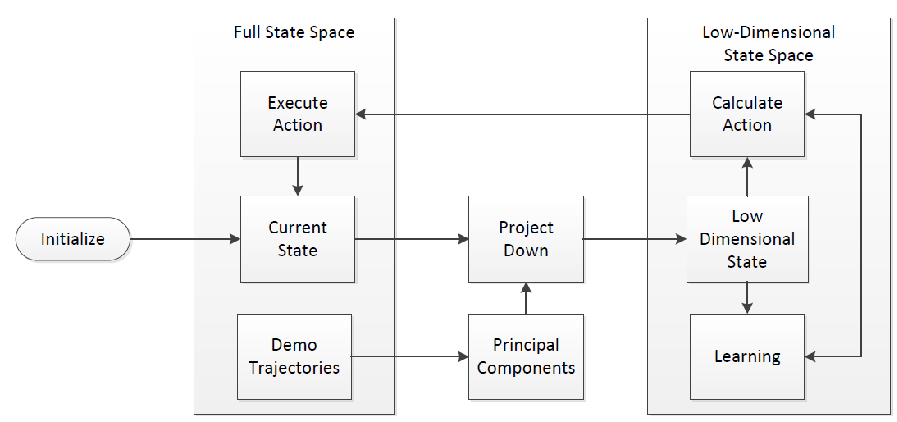
\includegraphics[width=0.38\textwidth]{Flowchart}
%  \caption{Approximation of RL combined with PCA.}
%  \label{fig:flowchart}
%\end{figure}


\subsection{Iterative DRRL}

%Work by \citeauthor{Grzes::mixed} \shortcite{Grzes::mixed} has shown that mixed resolution function approximation works well in complex domains. They build a function approximator that contains a coarse and finegrained representation, and learn both in parallel. In this way, they can quickly learn a good function approximation, and over time learn using a more expressive function to learn a high quality policy. We can leverage a similar idea in our iterative approach.

The key aspect of performing this iterative learning is transferring what was learned in the low-dimensional space to the high-dimensional space. To do this, we borrow from the field of transfer learning. In this work, we want to transfer all of the knowledge from the source to the target task. Additionally, the mapping from the source to the target task ($\chi_S(s)$) is given by PCA. This eases the transfer problem greatly. We only need to analyze when to transfer. If we transfer too early, the value function in the source domain is far from optimal. That bad knowledge can be spread throughout the value function in the target task.

To choose when to transfer, we borrow from the definition of convergence in Policy Iteration \cite{Sutton98reinforcementlearning}. In Policy Iteration, the value function is updated at each iteration until the policy does not change between updates. We make this policy comparison and ensure that the most recently executed policy is at least 95\% converged before transferring to the higher space.

Since IDRRL is a general technique, we can use any transfer learning approach within the constraints of the learning algorithm. Q-Value Reuse \cite{AAMAS07-taylor} is a simple technique applicable when the source and target task both use TD learning, as in our case. In Q-Value Reuse, a copy of the source task's value function is retained and used to calculate the target task's Q-Value. This computed Q-Value is a combination of the source task's saved value function and the target task's value function:

\begin{equation}
Q(s,a) = Q_{source}(\chi_S(s), \chi_A(a)) + Q_{target}(s,a)
\end{equation}
where $\chi$ is the transfer function between the source and target tasks' states and actions. This transfer function is the PCA projection. We then compute the Q-Learning update step as normal, but only the target's value function is updated. 

\subsection{Convergence Guarantees}

%Sample complexity measures the number of samples required for an RL algorithm to converge. The sample complexity is considered efficient if: within probability $1-\delta$, the RL algorithm is within $\epsilon$ of optimal on all but a polynomial number of steps. These polynomial steps are based on the size of the state space, the number of actions, $1/\delta$, $1/\epsilon$, $R_{max}$ and $\frac{R_{max}}{1-\gamma}$. Algorithms that are provably efficient with respect to sample complexity are called PAC-MDP(Brafman and Tennenholtz 2002; Ng, Harada, and Russell 1999; \cite{Strehl:2009:RLF:1577069.1755867}. 

%Although the learning algorithms have been proven to be PAC-MDP, the iterative transfer learning approach has not. Here, we show that by by transferring to the $n+1$ dimension we does not negate the PAC-MDP guarantees. We begin by analyzing the transfer approach.

Q-Value Reuse can be seen as a heuristic for action-value initialization. \citeauthor{Strehl:2009:RLF:1577069.1755867} \shortcite{Strehl:2009:RLF:1577069.1755867} demonstrated that if the action-values are admissible, then this initialization can decrease the sample complexity while maintaining PAC-MDP guarantees. Admissible heuristics provide valuable prior knowledge to PAC-MDP RL algorithms, but the specified prior knowledge does not need to be exact. An initialization heuristic ($H$) is said to be admissible if:

\begin{equation}
V^*(s) \leq Q^*(s,a) \leq H^*(s,a) \leq \frac{R_{max}}{1-\gamma}
\end{equation}
where $V^*(s)$ is the optimal value function, $Q^*(s,a)$ is the optimal action-value function, $H^*(s,a)$ is the initialization heuristic, and $\frac{R_{max}}{1-\gamma}$ is the maximum possible value. 

\citeauthor{Mann2012} \shortcite{Mann2012} extend PAC-MDP theory to intertask transfer learning. They introduce the concept of weakly admissible heuristics and show that they can still maintain PAC-MDP guarantees. To be weakly admissible, a heuristic needs to be admissible for only one action in each state. They combine weakly admissible heuristics and intertask mappings and prove they are also PAC-MDP given the following assumptions:

\begin{equation}
V^*_{trg}(s) - \alpha \leq Q^*_{trg}(s,\widetilde{a}) \leq Q^*_{src}(\chi_S(s), \chi_A(\widetilde{a}))
\end{equation}

Q-Learning is not originally PAC-MDP. However, we still enforce an admissible heuristic to make use of the \textit{optimism in the face of uncertainty} bias \cite{Brafman:2003:RGP:944919.944928}. This bias has been shown to reduce the chance of converging to a locally optimal policy. As it stands, Q-Value Reuse is not admissible. It is guaranteed to be less than $\frac{R_{max}}{1-\gamma}$, but is not greater than $Q^*(s,a)$.  We alleviate this issue by simply adding $R_{max}$ to each $Q_{source}(\chi_S(s), \chi_A(a))$ function. With IDRRL there is a risk of suboptimal convergence in a low-dimensional manifold biasing higher-dimensional learning. By forcing the Q-Reuse transfer heuristic to be admissible, we reduce, but not entirely eliminate this risk.

%TODO: Proof! Leverage + Rmax knowledge.

\section{Experimental Setup}
We wish to test the following hypotheses in this paper:

\begin{itemize}
\setlength\itemsep{0.01em}
\item $H1$: RL converges faster when combined with DRRL because of the smaller state representation. 
\item $H2$: RL converges to a locally optimal solution when combined with DRRL because of the less informative state representation.
\item $H3$: RL converges faster to a solution when combined with IDRRL without reducing performance.
\item $H4$: RL is robust to demonstration quality and number of demonstrations when combined with IDRRL.
\item $H5$: RL scales well with the size of the state space when combined with IDRRL.
\item $H6$: RL can efficiently take advatange of additional state information when combined with IDRRL.
\end{itemize}

We will test these hypotheses in the Mountain Car 3D, Mountain Car 4D, and Blackjack domains. For each experiment we use the following parameter settings for 20 statistical runs: $\alpha = 0.1$ and $\gamma = 0.99$.
\subsection{Mountain Car}
To test the efficacy of DRRL, we first consider the Mountain Car 3D domain. Mountain Car is a standard reinforcement learning domain \cite{NIPSbench:05}. In this problem an underpowered car must drive up a steep hill. The problem is engineered such that the car cannot overcome the effects of gravity, and cannot simply drive up the hill. Since the car starts in a valley, the agent must learn to build up enough inertia by driving partially up the opposite hill before it is able to make it to the goal.

In 2D Mountain Car, there are two states defined as the continuous position ($-1.2 \leq x \leq 0.6$) and velocity ($-.007 \leq v \leq .007$) of the car. There are three actions: Accelerate left, accelerate right, and neutral. The starting state is a random position at a random velocity. Lastly, the reward is -1 at each time step, and 100 at the goal. The 3D and 4D variant of Mountain Car are similar. There are two new states and actions for each additional dimension. 

\subsection{Blackjack}
Blackjack is a popular casino card game. The object of the game is to draw cards to get as close to 21 as possible. All digit cards are valued as the digit, the face cards count as 10, and the ace can be an 11 or 1. The game starts with two cards dealt to the dealer and the player. At this point the player can either hit (draw another card) or stay (finish) until they stay or exceed 21. If the player exceeds 21 it receives a reward of -1. The dealer then hits or stays based on a fixed strategy: he stays on a sum of 17 or greater, and hits otherwise. Once the dealer is done, if it exceeds 21, it loses and the agent receives a reward of 1. The player with the greater hand value wins. If there is a tie, the player receives a reward of 0, if the dealer wins the agent receives -1, and if the player wins the agent receives a 1.

The standard state representation for blackjack is defined as the player's hand value, the dealer's hand value, and whether or not the player has a usable ace \cite{NIPSbench:05}. If the player holds an ace that he could count as 11 without exceeding 21, then the ace is said to be usable.

\section{Results and Analysis}
We applied DRRL and IDRRL to three domains: Mountain Car 3D, Mountain Car 4D and Blackjack.

\subsection{Mountain Car}

In our formulation of Mountain Car we used 16 tiles and a $10^n$ tiling, where $n$ is the number of state variables. There are 4 state variables and 5 actions in the 3D variant, and 6 state variables and 7 actions in the 4D variant. We first learn using near-optimal demonstrations and single dimensions to test the efficacy of DRRL ($H1$). We also show that if the manifold does not represent enough variance in the data, the learning algorithm will converge to a suboptimal policy ($H2$). We then demonstrate that this issue is alleviated by IDRRL ($H3$). Lastly, we test the robustness of the demonstrations with respect to quality and performance ($H4$). We then use the Mountain Car 4D domain to show scalability ($H5$). To gather the demonstrations we learned good, bad, and random policies without our technique. We define good and bad policies by the reward they received during learning. Good demonstrations reached the goal within 300 time steps, and bad demonstrations within 500--1000 steps. Bad demonstrations reached the goal state, just less efficiently. 

There are two types of demonstrations we can use for PCA: one that explores the execution space, and one that performs a task. A demonstration that explores the execution space will gather more information about the entire state space than one which is targeted at performing a task.

In 3D and 4D Mountain Car there is no single state variable more important than all other state variables. Our PCA analysis shows that the first two principal components weigh all of the state variables equally, independent of demonstration quality. This is an example of execution space demonstrations. Even random demonstrations exploring the state space are useful in this scenario. 

Learning in only one manifold converged faster than learning in the full state space ($H1$, Figure \ref{fig:DRRL_3DMountainCar}). DRRL converged to the optimal solution using only 3 dimensions, rather than the full space of 4. It also converged to a near-optimal solution faster in only 2 dimensions. However, by using 2 dimensions, DRRL does not have a rich enough state space to learn optimally ($H2$).

\begin{figure}[h!]
  \centering
      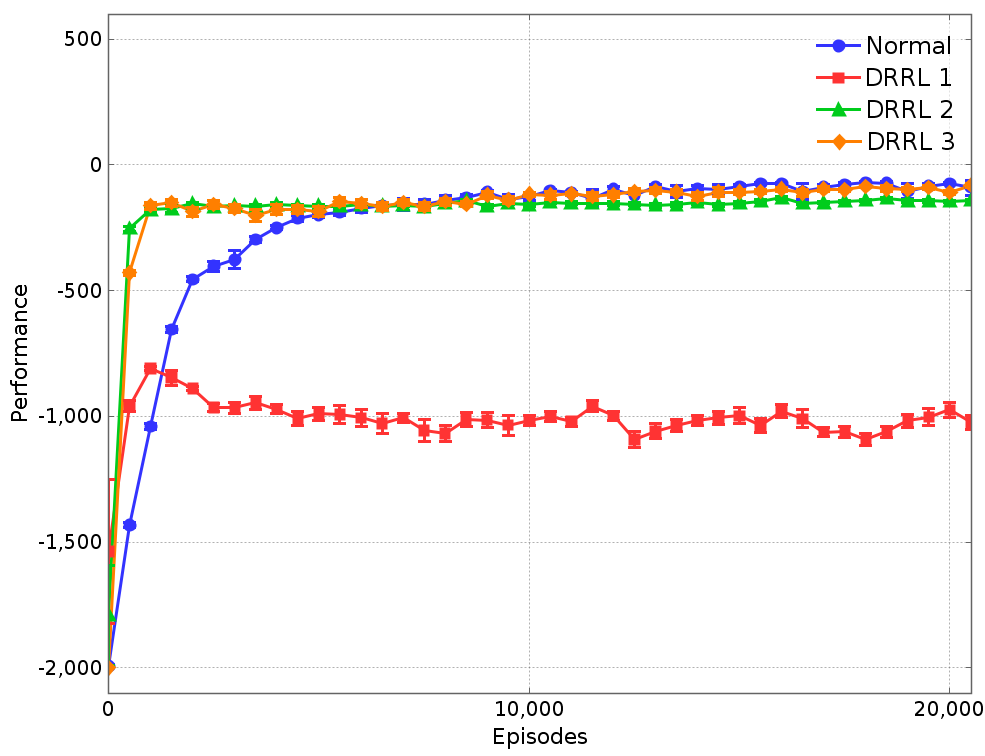
\includegraphics[width=0.38\textwidth]{DRRL_3DMountainCar}
  \caption{When using DRRL in Mountain Car 3D, two and three principal components converged quickly to a good, yet sub-optimal solution. The first principal component did not contain enough information to learn effectively.}
  \label{fig:DRRL_3DMountainCar}
\end{figure}

Combining standard reinforcement learning with IDRRL led the agent to converge faster with the same converged performance ($H3$, Figure \ref{fig:IDRRL_3DMountainCar}). DRRL converged slightly faster than IDRRL, but IDRRL benefits by using low variance but important states. Moreover, it does not require the algorithm designer to know beforehand which is the best manifold to learn in. 

Since IDRRL represents the state space in low-dimensional and sparse manifolds, it converges very quickly. With each additional manifold, it starts with a richer state space and the experience gained from all previous manifolds. By episode 2,000, IDRRL bootstrapped learning in the full dimensional space, and was near an optimal solution. This results in much faster convergence than learning entirely in the full dimensional space (Figure \ref{fig:IDRRL_3DMountainCar}).


\begin{figure}[h!]
  \centering
      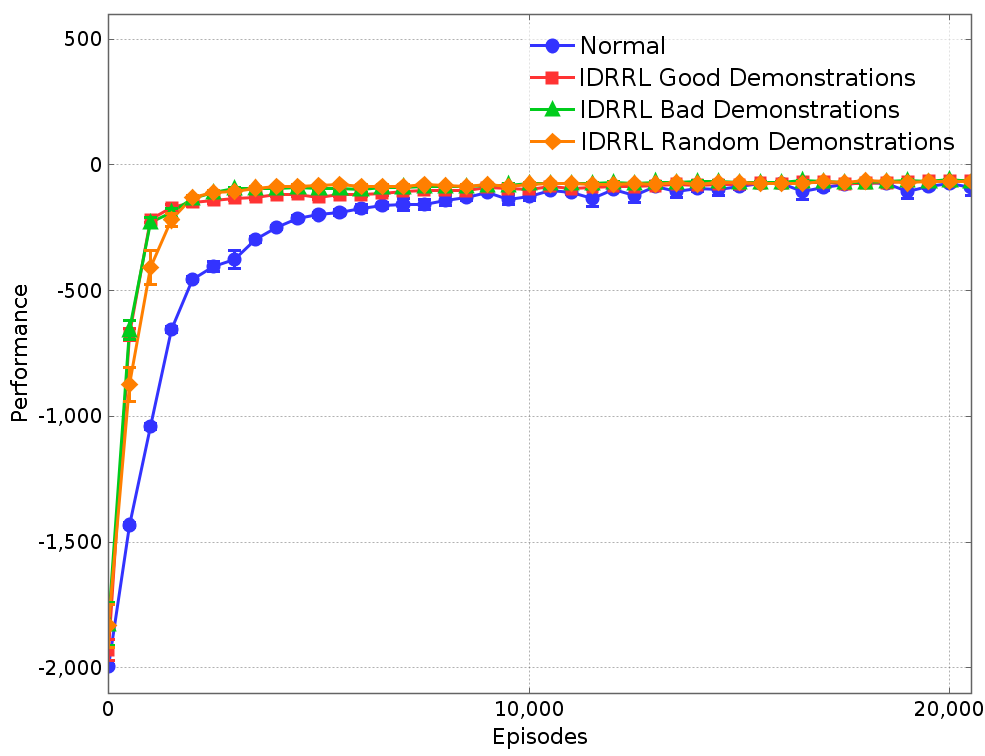
\includegraphics[width=0.38\textwidth]{IDRRL_3DMountainCar}
  \caption{IDRRL converged quickly to an optimal solution using standard Q-Learning. In Mountain Car 3D IDRRL is robust to suboptimal demonstrations.}
  \label{fig:IDRRL_3DMountainCar}
\end{figure}

To analyze the robustness of the approach ($H4$), we varied the quality of demonstration data as well as the amount. Figure \ref{fig:IDRRL_3DMountainCar} shows the relationship between demonstration quality and performance. There is no statistically significant difference between good, bad, and demonstrations. This is due to the equal weighing of all state variables.

To test $H4$ we also varied the amount of demonstration data. For this analysis, we used random demonstrations and varied the amount of demonstration data used between 1,000 and 25,000 demonstration points. All of the random demonstrations did not reach the goal state, and each demonstration was approximately 2,000 points. The experiment with 1,000 demonstration points converged slightly slower, and there were no statistically significant difference between 10,000 and 25,000 points.

\begin{figure}[h!]
  \centering
      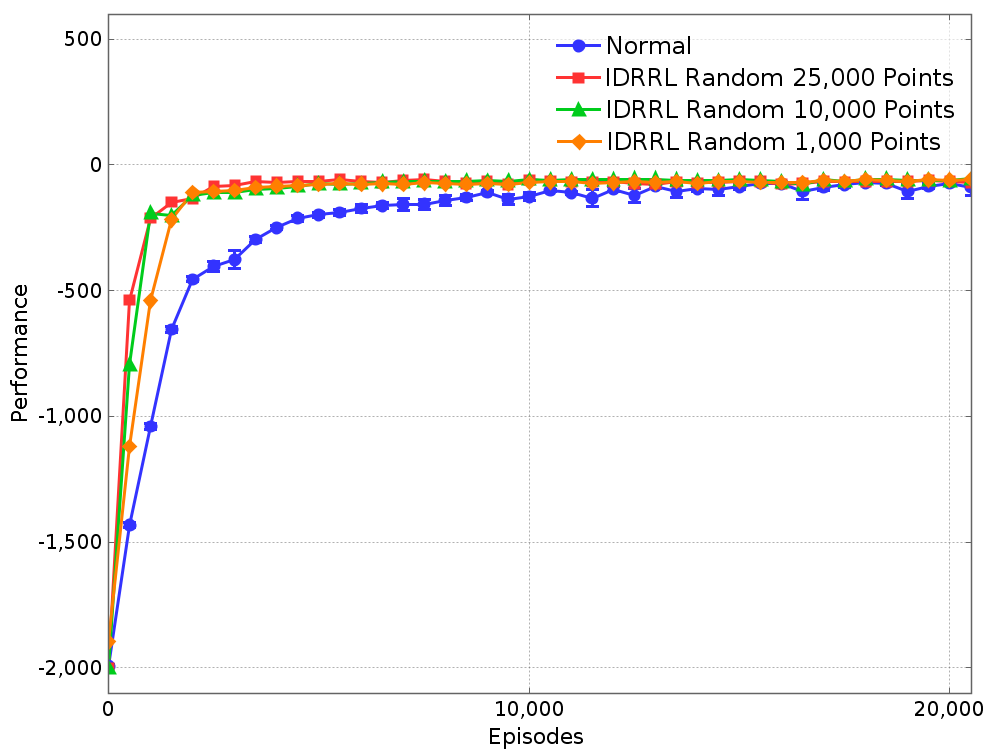
\includegraphics[width=0.38\textwidth]{IDRRL_Points_3DMountainCar}
  \caption{There is no statistically significant difference in performance between 10,000 and 25,000 demonstration points. }
  \label{fig:MC3D_GoodVarious}
\end{figure}


IDRRL also scales well with the size of the state space ($H5$). We modified Mountain Car 3D to add an additional fourth dimension. Mountain Car 4D has 6 continuous states and 7 actions. The performance trends seen in Mountain Car 3D are greater with the additional states (Figure \ref{fig:IDRRL_4DMountainCar}). By using IDRRL, the agent converges much faster to a good solution.

\begin{figure}[h!]
  \centering
      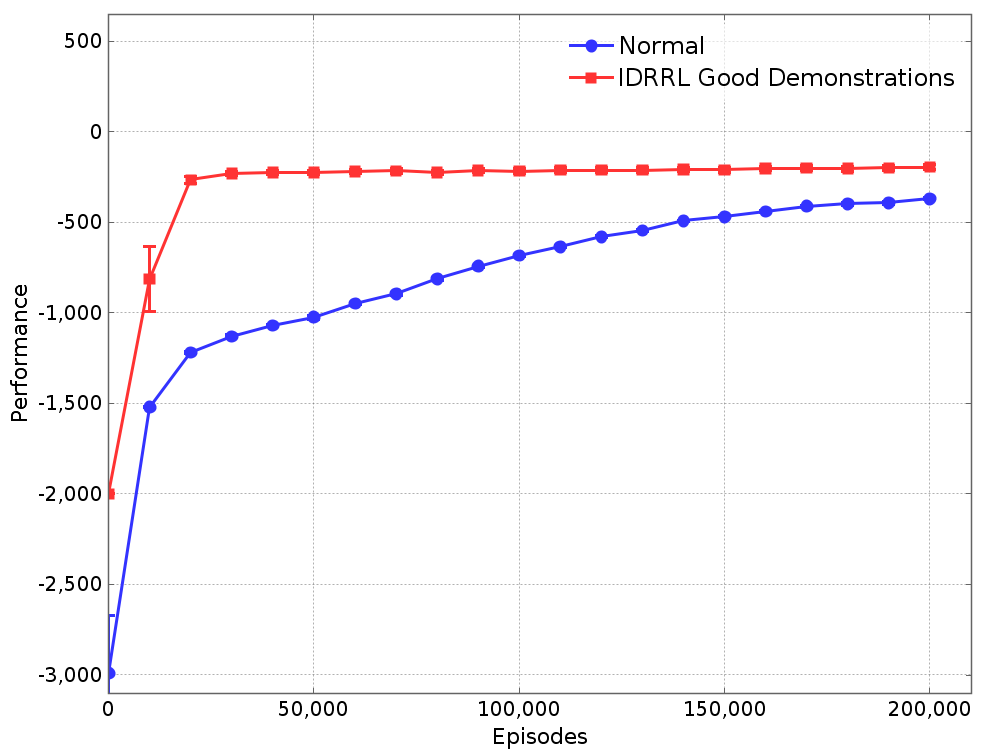
\includegraphics[width=0.38\textwidth]{IDRRL_4DMountainCar}
  \caption{In Mountain Car 4D, IDRRL scales well with the size of the state space.}
  \label{fig:IDRRL_4DMountainCar}
\end{figure}

\subsection{Blackjack}
Giving the agent additional helpful state variables makes convergence time longer, but can lead to a better solution. This is a standard cost-benefit analysis in reinforcement learning. The IDRRL approach makes it easy to add additional state information. IDRRL will initially learn using only a small amount of state information, and will add more once the solution has converged. Eventually, it will learn with all of the state information. We hypothesize the agent will learn faster than initially learning with all of the information ($H6$).

To show this, we taught a blackjack agent to count cards. In blackjack, it is well known that if the player knows the cards that are left in the deck, they have a large advantage. This also makes the amount of knowledge required to play blackjack greater. The player must keep track of the number of 13 different types of cards.

Originally blackjack had three states \cite{NIPSbench:05}, the player's hand value, the dealer's hand value, and whether or not the player has a usable ace. We add the number of aces, the number of cards valued between 2 and 5, the number of cards valued between 6 and 9, and the number of tens. 

We make the state representation for blackjack more complex so that better policies can be learned, but this leads to slower learning. Figure \ref{fig:Blackjack_IDRRL} shows that IDRRL can more efficiently take advantage of this new state information ($H6$). IDRRL initially performed worse due to 7 state variables being represented in a single dimension. Not enough variance was represented in this single state variable, and therefore the agent could not efficiently learn. As new state variables were added, IDRRL quickly began to out perform the standard approach.

\begin{figure}[h!]
  \centering
      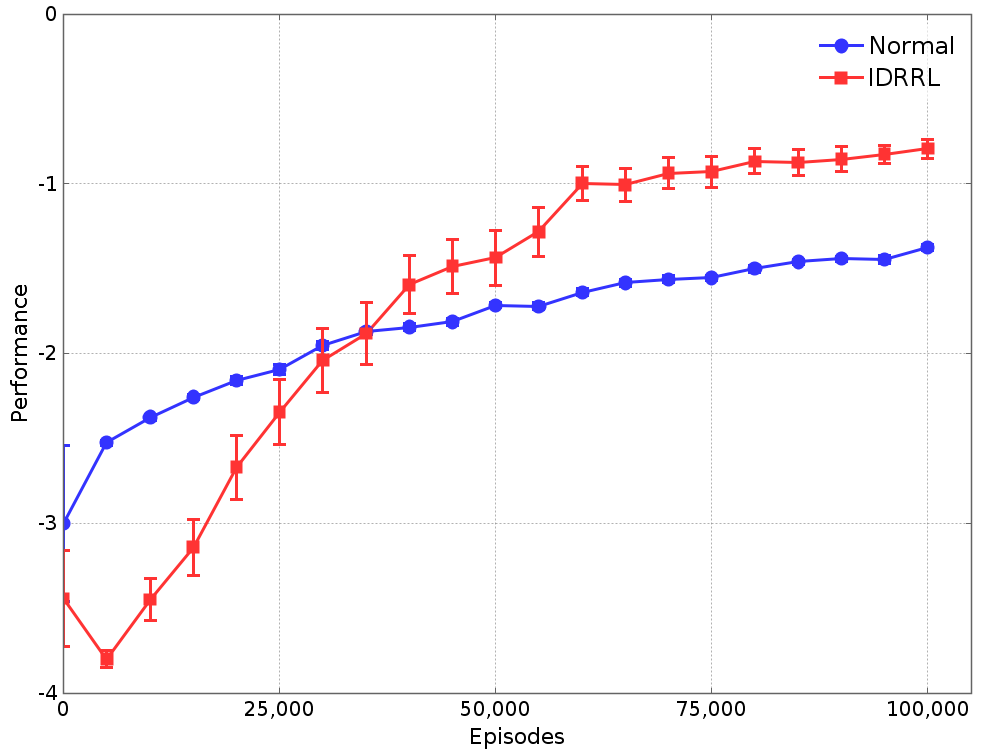
\includegraphics[width=0.38\textwidth]{Blackjack_IDRRL}
  \caption{By using IDRRL the blackjack agent efficiently used the additional state information.}
  \label{fig:Blackjack_IDRRL}
\end{figure}

\section{Conclusion and Future Work}
DRRL and IDRRL are not learning algorithms, but rather an addition to an existing learning algorithm. They improve the performance of an existing algorithm by combining the speed of low-dimensional learning and the expressiveness of the full state space. By projecting the state space onto a low-dimensional manifold, it is able to represent a complex state in only a few state variables. Then, by incrementally transferring the knowledge from low-dimensional spaces into the more complex spaces, IDRRL learns good policies very quickly. 

With IDRRL there is a risk of suboptimal convergence in a low-dimensional manifold biasing higher-dimensional learning. By forcing the Q-Reuse transfer heuristic to be admissible, we reduce, but not entirely eliminate this risk. Despite this fact, we show that IDRRL still converges to a good solution with 1,000 to 25,000 demonstration points.

In this work, the demonstrations spread across the execution space. When we ran PCA on those demonstrations, the first principal components weighed states with the least overall variance lowest. This was useful for learning with the most informative states early. However, if the demonstrations consist of solutions for a task, PCA will identify which states were not important for that specific task. This is extremely important when the execution space is large, and we want to teach the agent something specific.

In future work we would like to analyze task demonstrations for robotics. We hypothesize that by using IDRRL, the robot will learn efficiently. We also believe that learning with IDRRL will be robust to demonstration quality, a classic issue in learning from demonstration literature \cite{Argall:2009:SRL:1523530.1524008}. We also want to give the robot agent additional state information and see if it can efficiently leverage the new states and learn an effective policy.

IDRRL is independent of the learning algorithm, so we would like to combine it with a PAC-MDP algorithm. Fitted R-MAX is a variant of R-MAX, a PAC-MDP algorithm \cite{SARA07-jong}. It uses demonstration data to learn the transition probability distribution. By combining R-MAX with our IDRRL approach, we believe we can greatly improve performance.


\bibliographystyle{aaai}
\bibliography{thesis}
\end{document}